\documentclass{article}
\usepackage{microtype,graphicx,booktabs,amsmath,amssymb,hyperref}
\newcommand{\theHalgorithm}{\arabic{algorithm}}
\usepackage{icml2021}
\icmltitlerunning{Beyond Polynomial Expansion: Revisiting Kryptonite-3.0}
\begin{document}
\twocolumn[
\icmltitle{Beyond Polynomial Expansion: Revisiting Kryptonite-3.0 Through Representation, Data Scaling, and Low-Rank Adaptation}
\begin{icmlauthorlist}
\icmlauthor{Charlie Wang, Zihao Zhao, Jerry Li, William Chia}{imp}
\end{icmlauthorlist}
\icmlaffiliation{imp}{Imperial College London, London, United Kingdom}
\icmlcorrespondingauthor{Coursework team}{No email given}
\vskip 0.3in
]
\printAffiliationsAndNotice{}
\footnotetext{Development repository: \url{https://github.com/jerryliruijie/Kryptonite_v3.0}. Submission GitLab URL and final reproducible commit remain to be supplied.}

\begin{abstract}
Kryptonite-3.0 uses the failure of selected classifiers and frozen pretrained representations to argue that its tasks resist modern machine learning. We revisit this conclusion through representation-aware classification, matched learning-curve experiments, and low-rank adaptation (LoRA) of KryptoNet-40. On Kryptonite-20, -30, and -40, sign-transformed CatBoost achieves 94.58--95.42\% validation accuracy, compared with 52.75--53.86\% for quadratic logistic regression. Paired raw/sign experiments show that representation effects depend on the classifier. Quadrupling the training data improves sign-CatBoost by 7.03--13.92 percentage points, whereas the quadratic baseline gains at most 2.46 points. On Kryptonite-40-Adapt, rank-1 LoRA reaches 96.33\% mean validation accuracy across three seeds while training only 0.51\% of the model's parameters. These results challenge Kryptonite-3.0's general conclusions, showing that the failures of its selected methods do not extend to the alternative classifiers, data-scaling behaviour, and adaptation strategy evaluated here.
\end{abstract}

\section{Introduction}
Challenge datasets play an important role in evaluating the capabilities and limitations of machine learning models. However, poor performance on a particular benchmark does not necessarily indicate a fundamental limitation of machine learning. In practice, a model's performance depends on its expressive capacity, the effectiveness of optimization, and its ability to generalize to unseen data. Although universal approximation theorems establish that certain neural networks can approximate a broad class of functions, they do not guarantee successful training or generalization with finite data (Leshno et al., 1993). Consequently, the failure of a particular learning method should not be interpreted as evidence that a task is inherently unsolvable.

Kryptonite-3.0 (Quinn and Luther, 2026) challenges the effectiveness of machine learning through three main findings. First, polynomial logistic regression achieves less than 59\% accuracy even with polynomial features of degree 10, which the authors interpret as evidence against universal approximation. Second, quadrupling the training data produces only marginal improvements in quadratic logistic regression, leading the authors to question whether additional data can solve these tasks. Third, despite achieving 95\% accuracy on its pretraining task, KryptoNet-40 performs poorly under zero-shot evaluation and frozen-representation probing. However, these experiments examine a limited range of models and adaptation strategies. In particular, the failure of frozen representations does not establish whether updating the pretrained network could improve downstream performance.

To address these limitations, we systematically investigate alternative classification methods, the effects of training-set size, and parameter-efficient adaptation. We first compare logistic regression baselines with gradient-boosted decision trees and multilayer perceptrons (MLPs) trained from scratch. In particular, we examine how a sign-based input transformation affects the performance of different classifiers through controlled comparisons. We then investigate the relationship between training-set size and generalization by comparing learning curves on identical training subsets. Finally, we apply low-rank adaptation (LoRA) to KryptoNet-40, allowing its internal representations to be updated while keeping the pretrained hidden weights frozen.

Our main contributions are threefold:

\begin{enumerate}
\item \textbf{Representation-aware classification.} We demonstrate that alternative learning methods can achieve substantially higher accuracy than polynomial logistic regression on Kryptonite-3.0, and show that the effectiveness of sign-based representations depends on the classifier.
\item \textbf{Model-dependent data scaling.} Through matched learning-curve experiments, we show that increasing training data substantially improves sign-transformed CatBoost, in contrast to the limited gains observed for quadratic logistic regression.
\item \textbf{Parameter-efficient adaptation.} We demonstrate that LoRA enables effective adaptation of KryptoNet-40 under the evaluated setting, and provide a mathematical analysis of its trainable parameter count and computational complexity relative to full fine-tuning.
\end{enumerate}

\section{Methodology}
\subsection{Classification objective and polynomial controls}
For labelled observations $\mathcal D=\{(x_j,y_j)\}_{j=1}^m$, with $x_j\in\mathbb R^d$ and $y_j\in\{0,1\}$, a model produces a logit $z_\theta(x)$ and probability $p_\theta(x)=\sigma(z_\theta(x))$, where $\sigma(z)=(1+e^{-z})^{-1}$. We minimize binary cross-entropy,
\begin{equation}
\mathcal L=-\frac1m\sum_{j=1}^m\left[y_j\log p_j+(1-y_j)\log(1-p_j)\right].
\label{eq:bce}
\end{equation}
Logistic regression uses $z_\theta(x)=w^\top\phi(x)+b$. The linear control sets $\phi(x)=x$; the quadratic control includes the original coordinates and all products $x_i x_k$ for $i\leq k$. Its feature dimension is $d+d(d+1)/2$, excluding the intercept. Both use L2-regularized log loss, inverse regularization strength $C=0.85$, and L-BFGS with at most 1,000 iterations and tolerance $10^{-6}$. A training-majority classifier checks the approximately balanced task. These are shared-split controls, not a replication of Kryptonite-3.0's normalized degree-1--10 kernel experiment.

\subsection{Sign representations and tree ensembles}
Training-feature inspection identified coordinates concentrated near $-1$ and $+1$, motivating the fixed map
\begin{equation}
s_i(x)=\begin{cases}+1,&x_i\geq0,\\-1,&x_i<0.\end{cases}
\label{eq:sign}
\end{equation}
This discards magnitude variation; it creates no additional information and need not preserve all label-relevant structure. The supplied polynomial notebook also quantizes inputs, so the sign map itself is not our methodological novelty. The question is how a representation interacts with a learning algorithm.

CatBoost \cite{prokhorenkova2018} constructs an additive tree logit,
\begin{align}
F_t(s)&=F_{t-1}(s)+\eta T_t(s),\nonumber\\
p(x)&=\sigma(F_T(s(x))).
\end{align}
Successive trees reduce the regularized classification loss. We use 600 symmetric trees of depth 10, learning rate $\eta=0.05$, and leaf L2 regularization 10. Each symmetric tree applies a common split at each depth. Inputs are numerical sign values; the experiment does not establish a benefit from categorical-feature processing or ordered boosting.

To test whether sign preprocessing has a general benefit, we also hold fixed two contrasting tree classifiers. XGBoost \cite{chen2016} uses an additive boosted-tree logit with 200 depth-9 trees, learning rate 0.1 and L2 regularization 10. ExtraTrees \cite{geurts2006} averages class probabilities from 200 randomized trees, considers all features at each split, and uses minimum leaf size one without a depth cap. Each classifier is evaluated on both raw and sign inputs with the same folds and hyperparameters.

\subsection{MLPs and optimization}
The scratch MLP uses two ReLU hidden layers of equal width $h\in\{128,256\}$:
\begin{align}
h_1&=\operatorname{ReLU}(W_1\tilde x+b_1),\nonumber\\
h_2&=\operatorname{ReLU}(W_2h_1+b_2),\qquad z=w^\top h_2+b.
\end{align}
Here $\tilde x_i=(x_i-\mu_i)/\sigma_i$, with statistics fitted only on training rows. The model retains continuous magnitudes and learns its nonlinear representation, providing a complementary test to sign-based trees.

Adam \cite{kingma2015} uses gradient $g_t$, moment estimates $u_t=\beta_1u_{t-1}+(1-\beta_1)g_t$ and $v_t=\beta_2v_{t-1}+(1-\beta_2)g_t^2$, and the elementwise update
\begin{align}
\hat u_t&=\frac{u_t}{1-\beta_1^t},\qquad \hat v_t=\frac{v_t}{1-\beta_2^t},\nonumber\\
\theta_{t+1}&=\theta_t-\eta\frac{\hat u_t}{\sqrt{\hat v_t}+\epsilon}.
\end{align}
We use $(\beta_1,\beta_2)=(0.9,0.999)$, $\epsilon=10^{-8}$, $\eta=10^{-3}$ and batch size 256. Coupled weight decay adds $10^{-4}\theta_t$ to the loss gradient. Training runs for at most 150 epochs, with a minimum of 30 and patience 20 for validation-accuracy improvement. The checkpoint maximizes validation accuracy, with lower validation loss breaking ties.

\subsection{Low-rank adaptation of KryptoNet-40}
KryptoNet-40 has four width-512 ReLU hidden layers and a scalar output head, totalling 809,473 parameters. For a pretrained layer $W\in\mathbb R^{o\times i}$, LoRA \cite{hu2022} computes
\begin{equation}
Y=WX+b\mathbf1^\top+sBAX,\qquad s=\alpha/r,
\label{eq:lora}
\end{equation}
where $X\in\mathbb R^{i\times N}$, $A\in\mathbb R^{r\times i}$ and $B\in\mathbb R^{o\times r}$. We freeze $W,b$, initialize $A$ with Kaiming-uniform values and $B$ to zero, and train $A,B$. Thus the initial layer equals its pretrained counterpart, while $\operatorname{rank}(BA)\leq r$ constrains the update. We adapt all four hidden layers and train the existing output head, using raw inputs.

Writing $Z=AX$ and $G=\partial\mathcal L/\partial Y$, backpropagation gives
\begin{align}
\nabla_B\mathcal L&=sGZ^\top,& G_Z&=sB^\top G,\nonumber\\
\nabla_A\mathcal L&=G_ZX^\top,&\nabla_X\mathcal L&=W^\top G+A^\top G_Z.
\label{eq:gradients}
\end{align}
Initially $\nabla_A\mathcal L=0$, but $B$ can receive a nonzero gradient. Freezing $W$ removes its parameter gradient; it does not remove $W^\top G$ when gradients must reach earlier trainable layers.

\subsection{Training-step operation counts}
We count an $n\times m$ by $m\times k$ product as $nmk$ operations. One step means a forward and backward pass over $N$ inputs; bias additions, nonlinearities, scalar operations and optimizer updates are excluded. Full fine-tuning trains $oi+o$ parameters, including bias, and costs $3oiN$ if an input gradient is needed: $WX$, $GX^\top$ and $W^\top G$.

Evaluating $B(AX)$ and caching $Z$ costs $oiN+rN(i+o)$ forward operations. The parameter and intermediate gradients in Equation~\ref{eq:gradients} cost $rN(i+2o)$, and the input gradient costs $oiN+irN$. Consequently,
\begin{equation}
C_{\mathrm{LoRA}}=2oiN+3rN(i+o),\qquad
P_{\mathrm{LoRA}}=r(i+o).
\label{eq:cost}
\end{equation}
If the input gradient is unnecessary, the full and LoRA costs become $2oiN$ and $oiN+rN(2i+3o)$, respectively. The latter case applies to the first hidden layer when the input data require no gradient.

Product order matters in both passes. Forming $(BA)X$ costs $oir+oiN$ for the update alone, instead of $rN(i+o)$ for $B(AX)$. Similarly, computing $\nabla_A\mathcal L$ as $s(B^\top G)X^\top$ costs $rN(o+i)$, whereas $sB^\top(GX^\top)$ costs $oiN+roi$. Reusing $Z$ in $GZ^\top$ also avoids a dense intermediate. Efficient order depends on the dimensions and cached products; the factored order is appropriate for our small ranks.

Including the trainable 513-parameter head, the network has $3624r+513$ trainable parameters. Applying the appropriate first-layer count and including all later layers gives
\begin{align}
C_{\mathrm{full,net}}&=2{,}401{,}792N,\nonumber\\
C_{\mathrm{LoRA,net}}&=(1{,}594{,}880+10{,}832r)N.
\label{eq:networkcost}
\end{align}
At $r=1$, only 0.51\% of parameters are trained, but the counted operations remain 66.85\% of full fine-tuning. These are analytical matrix-operation counts, not measured speedups or energy savings.

\section{Experimental Design}
\subsection{Partitions and evaluation roles}
We use the supplied labelled datasets and shared stratified 70/20/10 train/validation/local-test partitions, with split seed 67 (Table~\ref{tab:data}). The training set is used for model fitting, while the validation set is used for hyperparameter tuning and checkpoint selection. The local test set is reserved for independent evaluation after model configurations have been finalized. Any data-dependent preprocessing is fitted exclusively on the corresponding training data to prevent information leakage. We use classification accuracy as the primary evaluation metric, with the 90\% threshold defined in the original paper serving as a reference for successful classification.



\begin{table}[t]
\centering
\begin{tabular}{lrrr}\toprule
Dataset & Train & Validation & Local test \\\midrule
K20 & 8,400 & 2,400 & 1,200 \\
K30 & 14,000 & 4,000 & 2,000 \\
K40 & 22,400 & 6,400 & 3,200 \\
K40-Adapt & 2,800 & 800 & 400 \\\bottomrule
\end{tabular}
\caption{Shared labelled-data partitions. The adaptation task has 40 input dimensions. Each separate hidden set has 10,000 unlabelled examples.}
\label{tab:data}
\end{table}

Model development is not identical across families. CatBoost's configuration was selected through K20 training-only three-fold cross-validation and then held fixed across datasets. The raw/sign ablation uses three stratified folds \emph{within the shared training partition}, with fold and model seed 67; its scores are separate from the outer validation scores. Earlier development informed the chosen classifiers and settings. MLP width is selected by mean outer validation accuracy over seeds 42, 123 and 2026. The same validation set selects MLP and LoRA checkpoints. Search budgets differ, so the study tests feasibility rather than equal-budget superiority.

To assess experimental variability, we report the sample standard deviation across three training seeds for MLP and LoRA, and across three cross-validation folds for the representation ablation. These measures reflect variability under their respective evaluation protocols rather than uncertainty across independent dataset splits. Model selection is performed using validation data, with local-test evaluation conducted only after the relevant models are finalized.

\begin{figure*}[t]
\centering
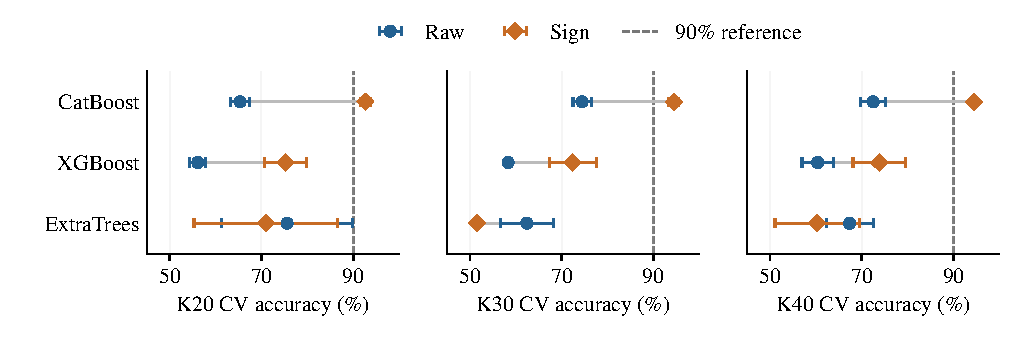
\includegraphics[width=\textwidth]{figures/representation.pdf}
\caption{Raw versus sign inputs for three fixed classifiers, evaluated by three-fold cross-validation inside the shared training partitions. Points are fold means; bars show one sample standard deviation across folds, not confidence intervals. Raw/sign conditions use identical folds and settings. The dashed 90\% line is a reference. These training-CV values are distinct from Table~\ref{tab:main}'s outer validation scores.}
\label{fig:representation}
\end{figure*}

\subsection{Hypotheses and controlled comparisons}
\textbf{H1: Alternative learning methods can overcome the limitations of polynomial classifiers.} Kryptonite-3.0 reports that polynomial logistic regression fails to reach its 90\% accuracy target, even with high-degree feature expansion. We investigate whether this limitation extends to other learning approaches by comparing majority, linear and quadratic logistic baselines with sign-transformed CatBoost and MLPs trained from scratch. To further examine the role of input representation, we conduct paired raw/sign comparisons across different classifiers while keeping their hyperparameters and cross-validation folds fixed. These experiments test whether alternative models can achieve strong classification performance and whether the benefits of sign-based representations depend on the learning algorithm.

\textbf{H2: The benefits of additional training data depend on the learning procedure.} Kryptonite-3.0 observes only marginal improvements when increasing the training data for quadratic logistic regression. To examine whether this finding generalizes, we compare its learning curve with that of sign-transformed CatBoost. Both methods are trained on identical nested subsets containing 25\%, 50\%, and 100\% of the available training data and evaluated on the same validation set, with hyperparameters fixed across training sizes. This comparison tests whether different learning procedures benefit differently from additional data, although it does not isolate the effects of model architecture and input representation.

\textbf{H3: LoRA can improve KryptoNet-40 adaptation beyond frozen-representation baselines.} Kryptonite-3.0 reports poor performance from zero-shot inference and frozen-feature probing, leaving adaptation of the pretrained hidden layers unexplored. We investigate whether updating these representations can improve downstream performance by comparing zero-shot KryptoNet-40, linear probing, and LoRA with ranks $(r\in\{1,2,4,8\})$ on Kryptonite-40-Adapt. Each trainable configuration is evaluated across three random seeds. LoRA adapts the hidden layers while retaining and training the pretrained output head, whereas the linear probe reinitializes its head and keeps the hidden layers frozen. Thus, the comparison evaluates the effectiveness of the complete adaptation strategies rather than isolating the contribution of hidden-layer updates alone.

\begin{figure*}[t]
\centering
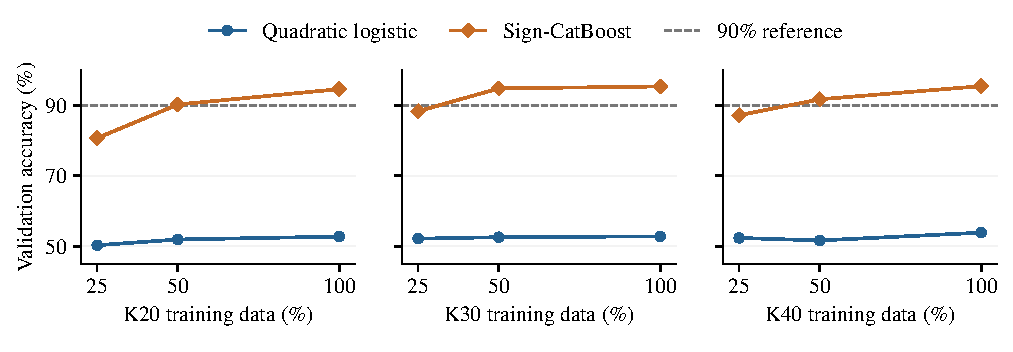
\includegraphics[width=\textwidth]{figures/learning_curves.pdf}
\caption{Validation accuracy on matched nested training subsets. Both methods use the same rows at each fraction and the same fixed validation set. Full training sizes are 8,400, 14,000 and 22,400 for K20, K30 and K40. Points represent single fits with fixed hyperparameters; connecting lines guide the eye and are not extrapolated scaling laws. The dashed line marks the 90\% reference.}
\label{fig:scaling}
\end{figure*}

\section{Experimental Results}
\subsection{Alternative classifiers exceed the polynomial controls}
Table~\ref{tab:main} reveals a substantial performance gap between the polynomial baselines and the nonlinear alternatives. While quadratic logistic regression performs only slightly above chance, sign-CatBoost exceeds the 90\% accuracy target on all three validation sets. This demonstrates that the poor performance of polynomial logistic regression does not extend to all learning methods, suggesting that the choice of representation and learning algorithm plays an important role in solving these tasks.


\begin{table}[t]
\centering
\begin{tabular}{lrrr}\toprule
Method & K20 & K30 & K40 \\\midrule
Majority & 50.42 & 50.05 & 50.19 \\
Linear logistic & 48.96 & 49.68 & 50.03 \\
Quadratic logistic & 52.75 & 52.80 & 53.86 \\
Sign-CatBoost & \textbf{94.58} & \textbf{95.33} & \textbf{95.42} \\
MLP (width 256) & 90.57 & 91.03 & 93.49 \\
\bottomrule
\end{tabular}

\caption{Accuracy (\%) on shared outer validation sets at full training size. MLP values average three seeds; all other entries are single fits. Bold marks the largest value in each column.}
\label{tab:main}
\end{table}

Importantly, strong performance is not limited to sign-transformed features. The MLP, trained directly on standardized continuous inputs, also achieves over 90\% mean validation accuracy across all three datasets. This provides complementary evidence that nonlinear models can learn the underlying classification patterns without explicitly applying the sign transformation. These results further support the ability of alternative models to generalize.

\subsection{Sign preprocessing has a model-dependent effect}
Figure~\ref{fig:representation} sharpens the interpretation of H1 by examining how input representations affect different classifiers. CatBoost benefits the most, achieving an improvement of over 20 percentage points across all three datasets, while XGBoost also shows consistent gains. These results suggest that sign-based representations are particularly effective for the tested gradient-boosted tree configurations, potentially making relevant feature interactions easier to learn.

However, this improvement does not generalize to all tree-based methods. ExtraTrees performs consistently worse after sign transformation, indicating that discarding feature magnitudes can also remove information useful to certain classifiers. Together, these contrasting results highlight the interaction between input representation and model inductive bias, rather than establishing sign transformation as a universally effective preprocessing strategy.

\subsection{Matched learning curves refute model-independent scaling failure}
Figure~\ref{fig:scaling} provides further evidence for H2 by revealing substantially different learning curves across the two methods. While quadratic logistic regression shows only marginal improvements as training data increases, sign-CatBoost benefits considerably from additional samples, exceeding the 90\ accuracy target on all three datasets with just 50\ of the available training data. This contrast suggests that the effectiveness of additional data depends on the learning procedure rather than being an inherent property of the dataset.

These findings directly challenge the broader conclusion drawn in Kryptonite-3.0. Although our quadratic baseline exhibits similarly limited improvements, the stronger scaling behaviour of sign-CatBoost demonstrates that this observation does not generalize to all learning methods. Nevertheless, the comparison involves different model families and input representations, and the observed trends over three training-set sizes do not establish a general scaling law.

\subsection{LoRA permits adaptation with few trainable parameters}
Table~\ref{tab:adapt} provides strong evidence for H3, showing that LoRA substantially outperforms both zero-shot inference and linear probing on Kryptonite-40-Adapt. While the frozen-representation baselines remain close to chance-level accuracy, all tested LoRA configurations exceed 95\ validation accuracy. These results challenge Kryptonite-3.0's conclusion that KryptoNet-40 cannot be effectively adapted, demonstrating that strong downstream performance is achievable when the pretrained network is updated through low-rank adaptation.

\begin{table}[t]
\centering
\begin{tabular}{lrr}\toprule
Method & Trainable params & Accuracy (\%) \\\midrule
Zero-shot & 0 & 49.00 \\
Linear probe & 513 & $52.42\pm0.31$ \\
LoRA $r=1$ & 4,137 & $96.33\pm0.07$ \\
LoRA $r=2$ & 7,761 & $95.67\pm1.23$ \\
LoRA $r=4$ & 15,009 & $96.29\pm0.19$ \\
LoRA $r=8$ & 29,505 & $96.17\pm0.19$ \\
\bottomrule
\end{tabular}

\caption{K40-Adapt validation accuracy on 800 examples. Trained methods report mean $\pm$ sample seed standard deviation (percentage points); zero-shot is deterministic.}
\label{tab:adapt}
\end{table}

Interestingly, increasing the LoRA rank does not consistently improve performance. Rank-1 LoRA achieves the highest mean validation accuracy while updating only 0.51\% of the model's parameters, suggesting that a compact low-rank update is sufficient to achieve strong performance under the evaluated setting. However, this does not establish that rank one is universally optimal, particularly as the scaling factor varies with rank.

\section{Discussion}
\subsection{Revisiting Kryptonite-3.0's inferences}
The three experiments support a connected rebuttal. Successful nonlinear classifiers show why failure of a selected polynomial learner cannot establish general unlearnability. The paired representation experiment identifies one important sensitivity without claiming a universal preprocessing remedy. Matched curves show that the usefulness of more data depends on the complete learning procedure. LoRA demonstrates that unsuccessful frozen probing cannot rule out adaptation that changes internal representations.

The theoretical inference fails independently of these empirical results. Universal approximation is an existence statement for a sufficiently rich function family under stated assumptions \cite{leshno1993}; it is not a guarantee about a particular degree cap, optimizer, regularization choice or finite training sample. Poor classification accuracy from a fitted polynomial model does not contradict that theorem. Equally, our successful fits do not prove it. The distinction between expressivity, optimization and generalization is essential to interpreting both studies.

\subsection{Limits and next experiments}
The generator remains unknown, and we do not infer a parity rule, noise model or unique causal mechanism from the observed feature distributions. Unequal tuning budgets, development reuse of validation data and one shared outer split limit general claims about model rankings. The raw/sign ablation controls representation within fixed classifiers, but does not explain all differences between CatBoost and the MLP. Independent evaluation of locked CatBoost and LoRA candidates, repeated outer splits, and matched head-initialization/learning-rate and layer-placement ablations would strengthen the evidence. Hidden-set success is not established by the present validation results.

\subsection{Environmental impact}
All recorded experiments ran on CPUs: Windows AMD machines for the baseline/tree experiments, an Apple M3 Pro for the MLPs, and a Qualcomm ARM CPU for adaptation. A partial runtime ledger contains 1.06 seconds for 15 baseline fits, 122.95 seconds for nine matched CatBoost fits, 1,145.85 seconds for 90 representation fits (including the wider five-classifier study), 73.51 seconds for 18 timed MLP run records, and 305.48 seconds for 21 adaptation records, including exploratory repeats. Timer scopes differ: fit-only, preprocessing-plus-fit, MLP run management, and adaptation training loops, respectively. These durations cannot support a fair speed ranking.

The ledger sums to 1,648.85 recorded seconds. Allocating an assumed 25--75 W to each recorded run gives a conditional energy scenario of $Pt/(3.6\times10^6)=0.0115$--$0.0344$ kWh. This is not measured consumption or a whole-project estimate: other searches, audits, untimed work and supplied pretraining are excluded, and concurrent runs may share a machine. We therefore do not estimate carbon emissions. Fixed transferred configurations, early stopping and reuse of recorded predictions limit repeated computation; LoRA reduces optimizer storage, while its energy benefit requires measurement.

\subsection{Conclusion}
Kryptonite-3.0 exposes limitations of particular learning procedures rather than establishing the broad impossibility claimed in Kryptonite-3.0. Representation-aware classification, matched data-scaling experiments and low-rank internal adaptation provide concrete counterevidence. The defensible conclusion is that those failures do not generalize to the alternatives tested here; final challenge success still requires evaluation of locked predictions on the hidden sets.

\clearpage
\begin{thebibliography}{9}
\bibitem[Chen and Guestrin(2016)]{chen2016}
Chen, T. and Guestrin, C.
XGBoost: A scalable tree boosting system.
In \emph{Proceedings of the 22nd ACM SIGKDD International Conference on Knowledge Discovery and Data Mining}, pp.\ 785--794, 2016.
\url{https://doi.org/10.1145/2939672.2939785}.

\bibitem[Geurts et al.(2006)]{geurts2006}
Geurts, P., Ernst, D., and Wehenkel, L.
Extremely randomized trees.
\emph{Machine Learning}, 63:3--42, 2006.
\url{https://doi.org/10.1007/s10994-006-6226-1}.

\bibitem[Hu et al.(2022)]{hu2022}
Hu, E. J., Shen, Y., Wallis, P., Allen-Zhu, Z., Li, Y., Wang, S., Wang, L., and Chen, W.
LoRA: Low-rank adaptation of large language models.
In \emph{International Conference on Learning Representations}, 2022.
\url{https://arxiv.org/abs/2106.09685}.

\bibitem[Kingma and Ba(2015)]{kingma2015}
Kingma, D. P. and Ba, J.
Adam: A method for stochastic optimization.
In \emph{International Conference on Learning Representations}, 2015.
\url{https://arxiv.org/abs/1412.6980}.

\bibitem[Leshno et al.(1993)]{leshno1993}
Leshno, M., Lin, V. Y., Pinkus, A., and Schocken, S.
Multilayer feedforward networks with a nonpolynomial activation function can approximate any function.
\emph{Neural Networks}, 6(6):861--867, 1993.
\url{https://doi.org/10.1016/S0893-6080(05)80131-5}.

\bibitem[Prokhorenkova et al.(2018)]{prokhorenkova2018}
Prokhorenkova, L., Gusev, G., Vorobev, A., Dorogush, A. V., and Gulin, A.
CatBoost: Unbiased boosting with categorical features.
In \emph{Advances in Neural Information Processing Systems}, volume 31, 2018.
\href{https://proceedings.neurips.cc/paper/2018/hash/14491b756b3a51daac41c24863285549-Abstract.html}{NeurIPS 2018 proceedings}.

\bibitem[Quinn and Luther(2026)]{quinn2026}
Quinn, H. and Luther, L.
Kryptonite-3.0: The final end to machine learning hype?
Mathematics for Machine Learning coursework mock paper, Imperial College London, 2026.
\end{thebibliography}
\end{document}
